\section*{Введение}
\addcontentsline{toc}{section}{\protect Введение}%
IN PROGRESS...


\section{Описание конструкции реактора}
IN PROGRESS...



\section{Теплофизический расчет}

\subsection{Постановка задачи}
В данном разделе будут определены основные термодинамические и гидравлические параметры реакторной установки. Теплофизический расчет подразумевает следующий ряд задач:

    \begin{enumerate}
        \item Выбор турбины и разработка принципиальной теплосиловой схемы установки;
        \item Рассчет КПД проектируемой установки;
        \item Рассчет основных теплофизических характеристик, таких как мощность ТВС и твэла, расход и скорсоть теплоносителя, коэффициент теплоотдачи;
        \item Построение распределения температур теплоносителя, оболочки и топлива по длинне для наиболее напряжённого канала; 
        \item Определение максимально возможных температур теплоносителя, оболочки и топлива;
        \item Рассчёт энергозатраты на собственные нужды и уточнение КПД;
        \item Рассчёт коэффициента запаса до кризиса теплообмена;
    \end{enumerate}

\subsection{Исходные данные для проведения расчетов}


Для проведения теплогидравлического расчета реакторной установки использовались следующие характеристики, представленные в Таблице \ref{tabular:data}.

\begin{table}[H]
	\caption{Исходные данные для проектируемого РУ ВВЭР-1000}
	\begin{center}
        \begin{tabular}{|l|c|}
        \toprule
         Характеристика & Значение \\ 
         \midrule
         \hline
         Электрическая мощность реактора, МВт & 1000 \\
         \hline\ 
         Температура теплоносителя на входе в АЗ $T_{\text{вх}}$, $^\circ C$  & 287 \\ 
         \hline\
         Температура теплоносителя на выходе АЗ $T_{\text{вых}}$, $^\circ C$ & 320 \\ 
         \hline
         Температура питательной воды, , $^\circ C$ & 220 \\ 
         \hline
         Температура свежего пара, $^\circ C$  &  281 \\ 
         \hline
         Давление свежего пара & 6.5 \\ 
         \hline
         Температура пара после пароперегревателей, $^○C$ & 250 \\ 
         \hline
         Давление в АЗ, МПа & 15.7 \\ 
         \hline
         Степень сухости пара прсле ЦВД и ЦНД, \% & 80 \\ 
         \hline
         Количество петель РУ & 4 \\ 
         \hline
         Число ТВС $N_{\text{ТВС}}$, шт  & 163 \\ 
         \hline
         Число твэл в ТВС $N_{\text{твэл}}$, шт & 317 \\ 
         \hline
         Коэффициент неравномерности по высоте АЗ  & 1.5 \\ 
         \hline
         Коэффициент неравномерности по радиусу АЗ & 1.25 \\ 
         \hline
         Высота АЗ $H_{\text{AZ}}$, м & 3.5 \\ 
         \hline
         Диаметр твэл $d_{\text{тв}}$, мм & 9.1 \\ 
         \hline
         Размер ТВС «под ключ» $a$, мм & 234 \\ 
         \hline
         Диаметр центрального канала в ТВС $D_{\text{ц.к}}$, мм & 10.3 \\ 
         \hline
         Число направляющих каналов в ТВС $N_{\text{н.к.}}$, шт & 12 \\ 
         \hline
         Шаг решетки ТВС $S_m$, мм & 12,75 \\ 
         \hline
         Диаметр направляющего канала в ТВС $D_{\text{н.к}}$, мм & 12.6 \\ 
         \hline
         Толщина оболочки твэл $\delta_{\text{твэл}}$, мм & 0.65 \\ 
         \hline
         Толщина газового зазора в твэл $\delta_{\text{г}}$, мм & 0.135 \\ 
         \hline
         Диаметр топливной таблетки $d_{\text{топ}}$, мм. & 7.53 \\ 
         \hline
         Диаметр отверстия топливной таблетки $d_{\text{\text{отв}}}$, мм & 1.3 \\ 
        %  \hline
        %  Число СУЗ $N_{\text{СУЗ}}$, шт & 109 \\ %сомнительная штука https://ru.wikipedia.org/wiki/%D0%92%D0%92%D0%AD%D0%A0-1000
        %  \hline
        %  Диаметр СУЗ $D_{\text{СУЗ}}$, мм & 8.2 \\
         \bottomrule
		\end{tabular}
		\label{tabular:data}
	\end{center}
\end{table}




\subsection{Выбор турбины}
В качестве турбины в расчетах будем использовать модель К-1000-60/1500-2. Её характеристики представлены в таблице \ref{tabular:turbine}


\begin{table}[H]
	\caption{Параметры турбины К-1000-60/1500-2 }
	\begin{center}
        \begin{tabular}{|l|c|}
        \toprule
         Параметр & Значение или Название \\ 
         \midrule
         \hline
         Прототип турбины &  К-1000-60/1500\\ 
         \hline
         Температура питательной воды, $^\circ C$ & 220 \\ 
         \hline
         Температура свежего пара, $^\circ C$  & 281\\ 
         \hline
         Давление свежего пара, $^\circ C$ & 6.5 \\ 
         \hline
         Температура после промежуточного перегрева, $^○C$ & 250 \\ 
         \hline
         Количество регенеративных подогревателей & 7 \\ 
         \bottomrule
		\end{tabular}
		\label{tabular:turbine}
	\end{center}
\end{table}


\begin{figure}[H]
	\begin{center}
		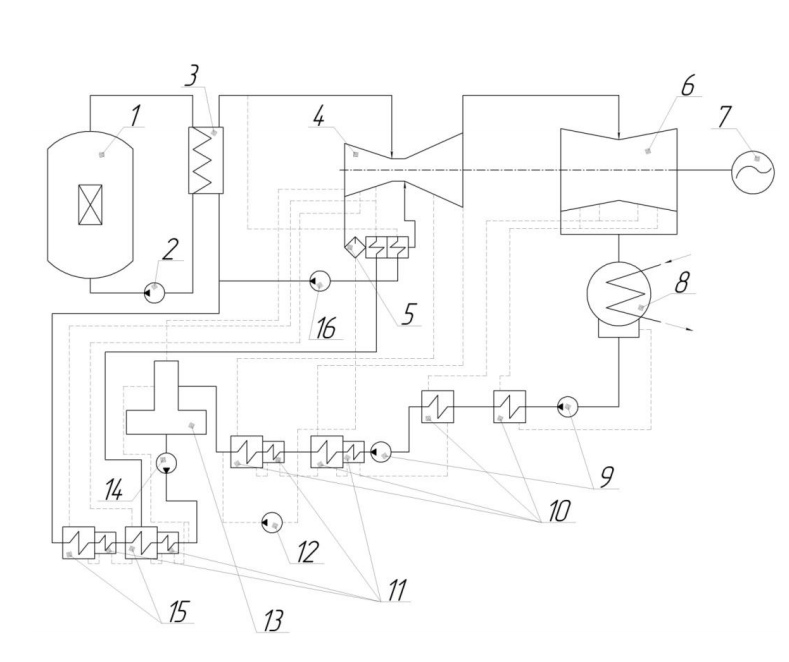
\includegraphics[scale=0.5]{teploscheme.jpg}
		\caption{Тепловая схема АЭС: 1 – ядерный реактор, 2 – главный
циркуляционный насос, 3 – парогенератор, 4 – цилиндр высокого давления, 5 –
сепаратор-пароперегреватель, 6 – цилиндры низкого давления, 7 – генератор, 8
– конденсатор, 9 – конденсационный электронасос, 10 – подогреватель низкого
давления, 11 – охладитель, 12 – станция насосная, 13 – деаэратор, 14 –
плунжерный электронасос, 15 – подогреватель высокого давления, 16 –
конденсационный насос с гидротурбинным приводом}
		\label{pic:teplocheme} % название для ссылок внутри кода
	\end{center}
\end{figure}


\subsection{Расчет КПД термодинамического цикла}


\begin{figure}[H]
	\begin{center}
		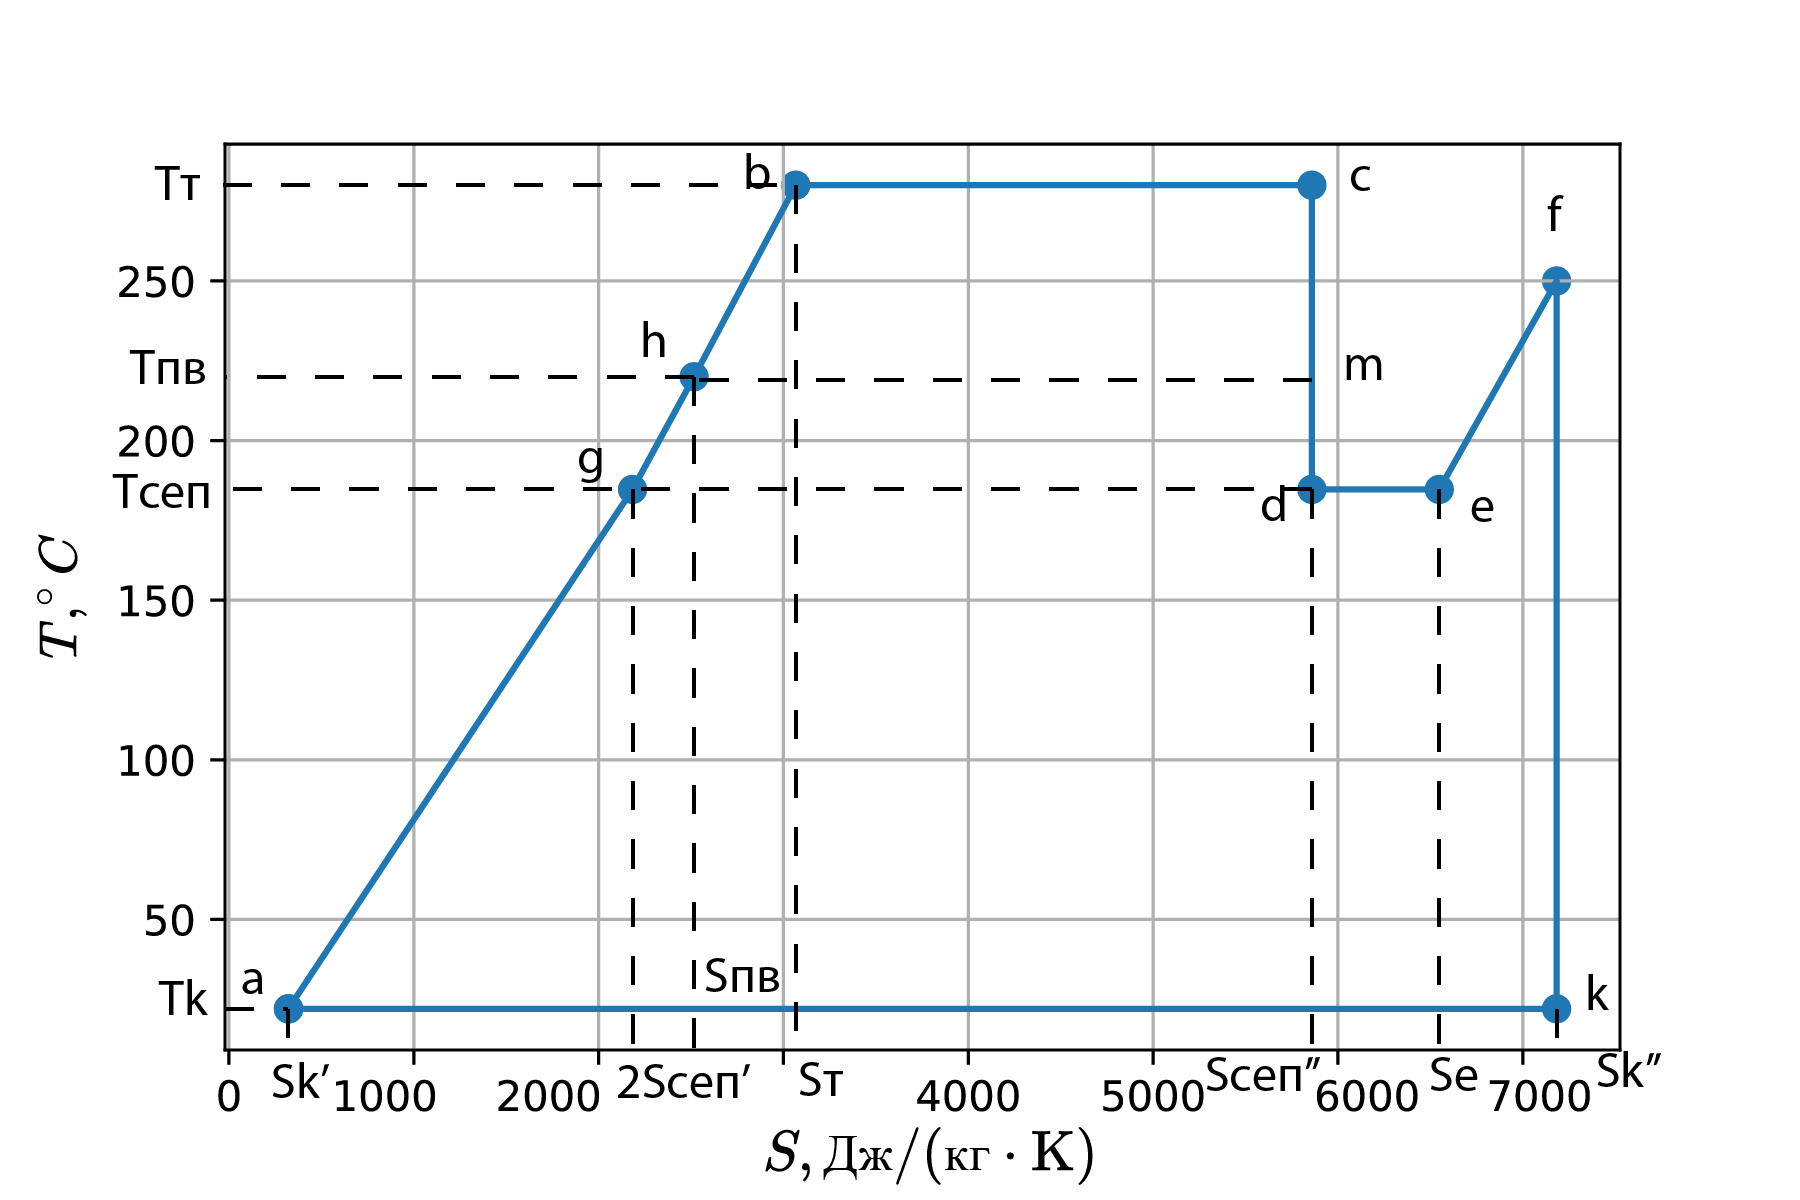
\includegraphics[scale=0.15]{TS.png}
		\caption{ T­S диаграмма турбинного цикла в реакторе ВВЭР­1000 : hbc —нагрев и испарение в парогенераторе; cd — расширение пара в ЦВД; de — паротделяется от конденсата в сепараторе; ef — пар поступает в промежуточныйпароперегреватель; fk — расширение пара в ЦНД; ka ­ конденсация в конден­саторе; ag — регенеративный подогрев в ПНД; gh — регенеративный подогревв ПВД6
        }
		\label{pic:TS} % название для ссылок внутри кода
	\end{center}
\end{figure}

\begin{table}[H]
	\caption{Значения параметров TS-диаграммы}
	\begin{center}
        \begin{tabular}{|c|c|c|c|c|}
        \toprule
         Точка & P, МПа & T, $^\circ C$ & S, Дж/(кг*К) & h, кДж/кг \\ 
         \midrule
         \hline
          h &  2.6 & 220 & 2517 & 943.7\\ 
         \hline
          b & 6.5 & 281 & 3076 & 2780 \\ 
         \hline
          c & 6.5 & 281 & 5852 & 2779\\ 
         \hline
          d & 1.13 & 185 & 5852 & 2465 \\ 
         \hline
          e & 1.13 & 185 & 6543 & 2782 \\ 
         \hline
          f & 1.13 & 250  & 6863 & 2938 \\ 
         \hline
          k & 0.0023 & 20 & 6863 & 1998 \\ 
         \hline
          k′ & 0.0023 & 20 & 295.2 & 83.92 \\ 
         \hline
          a & 6.5 & 20 & 295.2 & 90 \\ 
         \hline
          g & 1.13 & 185 & 2188 & 785.3 \\ 
         \bottomrule
		\end{tabular}
		\label{tabular:coeffs}
	\end{center}
\end{table}

Произведём расчет КПД для турбины К-1000-60/1500. Термический КПД без регенерации:
$$
η_{t0} = 1 -
\frac{T_{k} ⋅ \left( s_{f} - s_{a} \right) ⋅ x_{d}}
{\left( h_{c} - h_{g} \right) +x_{d}\left( \left( h_{g} - h_{a} \right) + \left( h_{f} - h_{e} \right) \right)} = 0.424
%= \VAR{KPD_t0}
$$
Термический КПД с идеальной регенерацией:
$$
η_{t∞} = 1 -
\frac{T_{k} ⋅ \left( s_{f} - s_{g} \right) \left( s_{c} - s_{h} \right)}
{\left(h_{c} - h_{h}\right) ⋅ \left( s_{e} - s_{g} \right) + \left( h_{f} - h_{e} \right) ⋅ \left( s_{f} - s_{h} \right)} = 0.473
%= \VAR{KPD_t∞}
$$
Термический КПД с $n = 7$  регенеративными отборами:
$$
η_{tn} = η_{t0} + \left( η_{t∞} - η_{t0} \right) ⋅ \frac{n}{n+1} = 0.467
%= \VAR{KPD_tn}
$$

Учитываем:
$\eta^{\text{вн}}$ = 0.85 — внутренний КПД турбины;
$\eta_{\text{ос}}$ = 0.98 — коэффициент использования тепла, учитывающий; потери тепла в окружающую среду в прочем энергооборудовании;
$\eta_{\text{эг}}$ = 0.98 — КПД электрогенератора;
$\eta_{\text{мех}}$ = 0.97 — КПД механический,
Вычисляем КПД брутто АЭС как:
$$
\eta_{\text{брутто}} = \eta^7 \cdot \eta^{\text{вн}} \cdot \eta_{\text{ос}} \cdot \eta_{\text{эг}} \cdot \eta_{\text{мех}} = 0.37
$$
Тепловая мощность реактора при номинальной электрической мощности $Q_{\text{эл}} = 1000$ МВт равна:
$$
Q_{\text{теп}} = \frac {Q_{\text{эл}}} {\eta^{\text{брутто}}} = 2700 МВт 
$$


\subsection{Расчет изменения теплового потока в наиболее нагруженном канале}
Из условия $K_z = \frac 1 {\int_{-H_{\text{аз}}/2}^{H_{\text{аз}}/2} \cos \left( \frac {\pi \cdot z} {H_{\text{эф}}}\right)dz} = 1.5$ находим эфективную добавку к высоте активной зоны. Эффективная высота активной зоны будет равна $H_{\text{эф}} = 2.66$ м. Максимальная величина теплового потока на один твэл:
$$
q_{max} = \frac {Q_{\text{теп}}K_r K_z}{N_{ТВС}N_{\text{твэл}}H_{\text{аз}}} = 279.93\  \frac {\text{Вт}} {\text{см}}
$$ 
Зависимость величины теплового потока от высоты:
$$
q(z) = q_{max}\cos\left(\frac {\pi\cdot z} {H_{\text{эф}}}\right) = 279.93 \cos \left(\frac {\pi \cdot z} {266} \right)\ \left[\frac{\text{Вт}}{\text{см}} \right]
$$

\subsection{Расчет распределения температуры теплоносителя по высоте}

Энтальпия входа $h_{\text{вх}} =1.268 \cdot 10^6 \frac{Дж}{кг}$.%из wsp через F(P,T) температуру на входе и давление в АЗ.

\noindent Энтальпия выхода $h_{\text{вых}} =1.453 \cdot 10^6 \frac{Дж}{кг}$. %аналогично 

\noindent Расход теплоносителя через ТВС:
$$
G_{ТВС} = \frac {Q_{\text{теп}}} {(h_{\text{вх}} - h_{\text{вх}})N_{\text{ТВС}}} = 89.67 \ \frac {\text{кг}}{\text{c}} 
$$
Расход теплоносителя через реактор:
$$
G_{\text{реак}} = \frac {Q_{\text{теп}}} {\left(h_{\text{вых}} - h_{\text{вх}}\right)} = 14615.6\ \frac{\text{кг}} {\text{с}}
$$
Средняя теплоемкость воды:
$$
C_p = \frac {h_{\text{вых}} - h_{\text{вх}}} {T_{\text{вых}} - T_{\text{вх}}} = 5606.06\ \frac{\text{Дж}} {\text{кг} \cdot \text{К}}
$$
\noindent Распределение температуры теплоносителя по высоте реактора:
$$
T_{ТН}(z) = T_{\text{вх}} + \frac {N_{\text{ТВС}}N_{\text{ТВЭЛ}}q_{\max}H_{\text{эф}}} {G_{\text{реак}}C_p\pi}\left[\sin \left(\frac {\pi z}{H_{\text{эф}}} \right) +\sin \left(\frac {\pi H_{\text{АЗ}}} {2H_{\text{эф}}} \right) \right]
$$
\noindent Отсюда максимальная температура жидкости $T_{\text{ТН}}^{max} = 315.092\  ^\circ C$.
График изменения температуры теплоносителя по высоте представлен на \ref{pic:TZ}

\begin{figure}[H]
	\begin{center}
		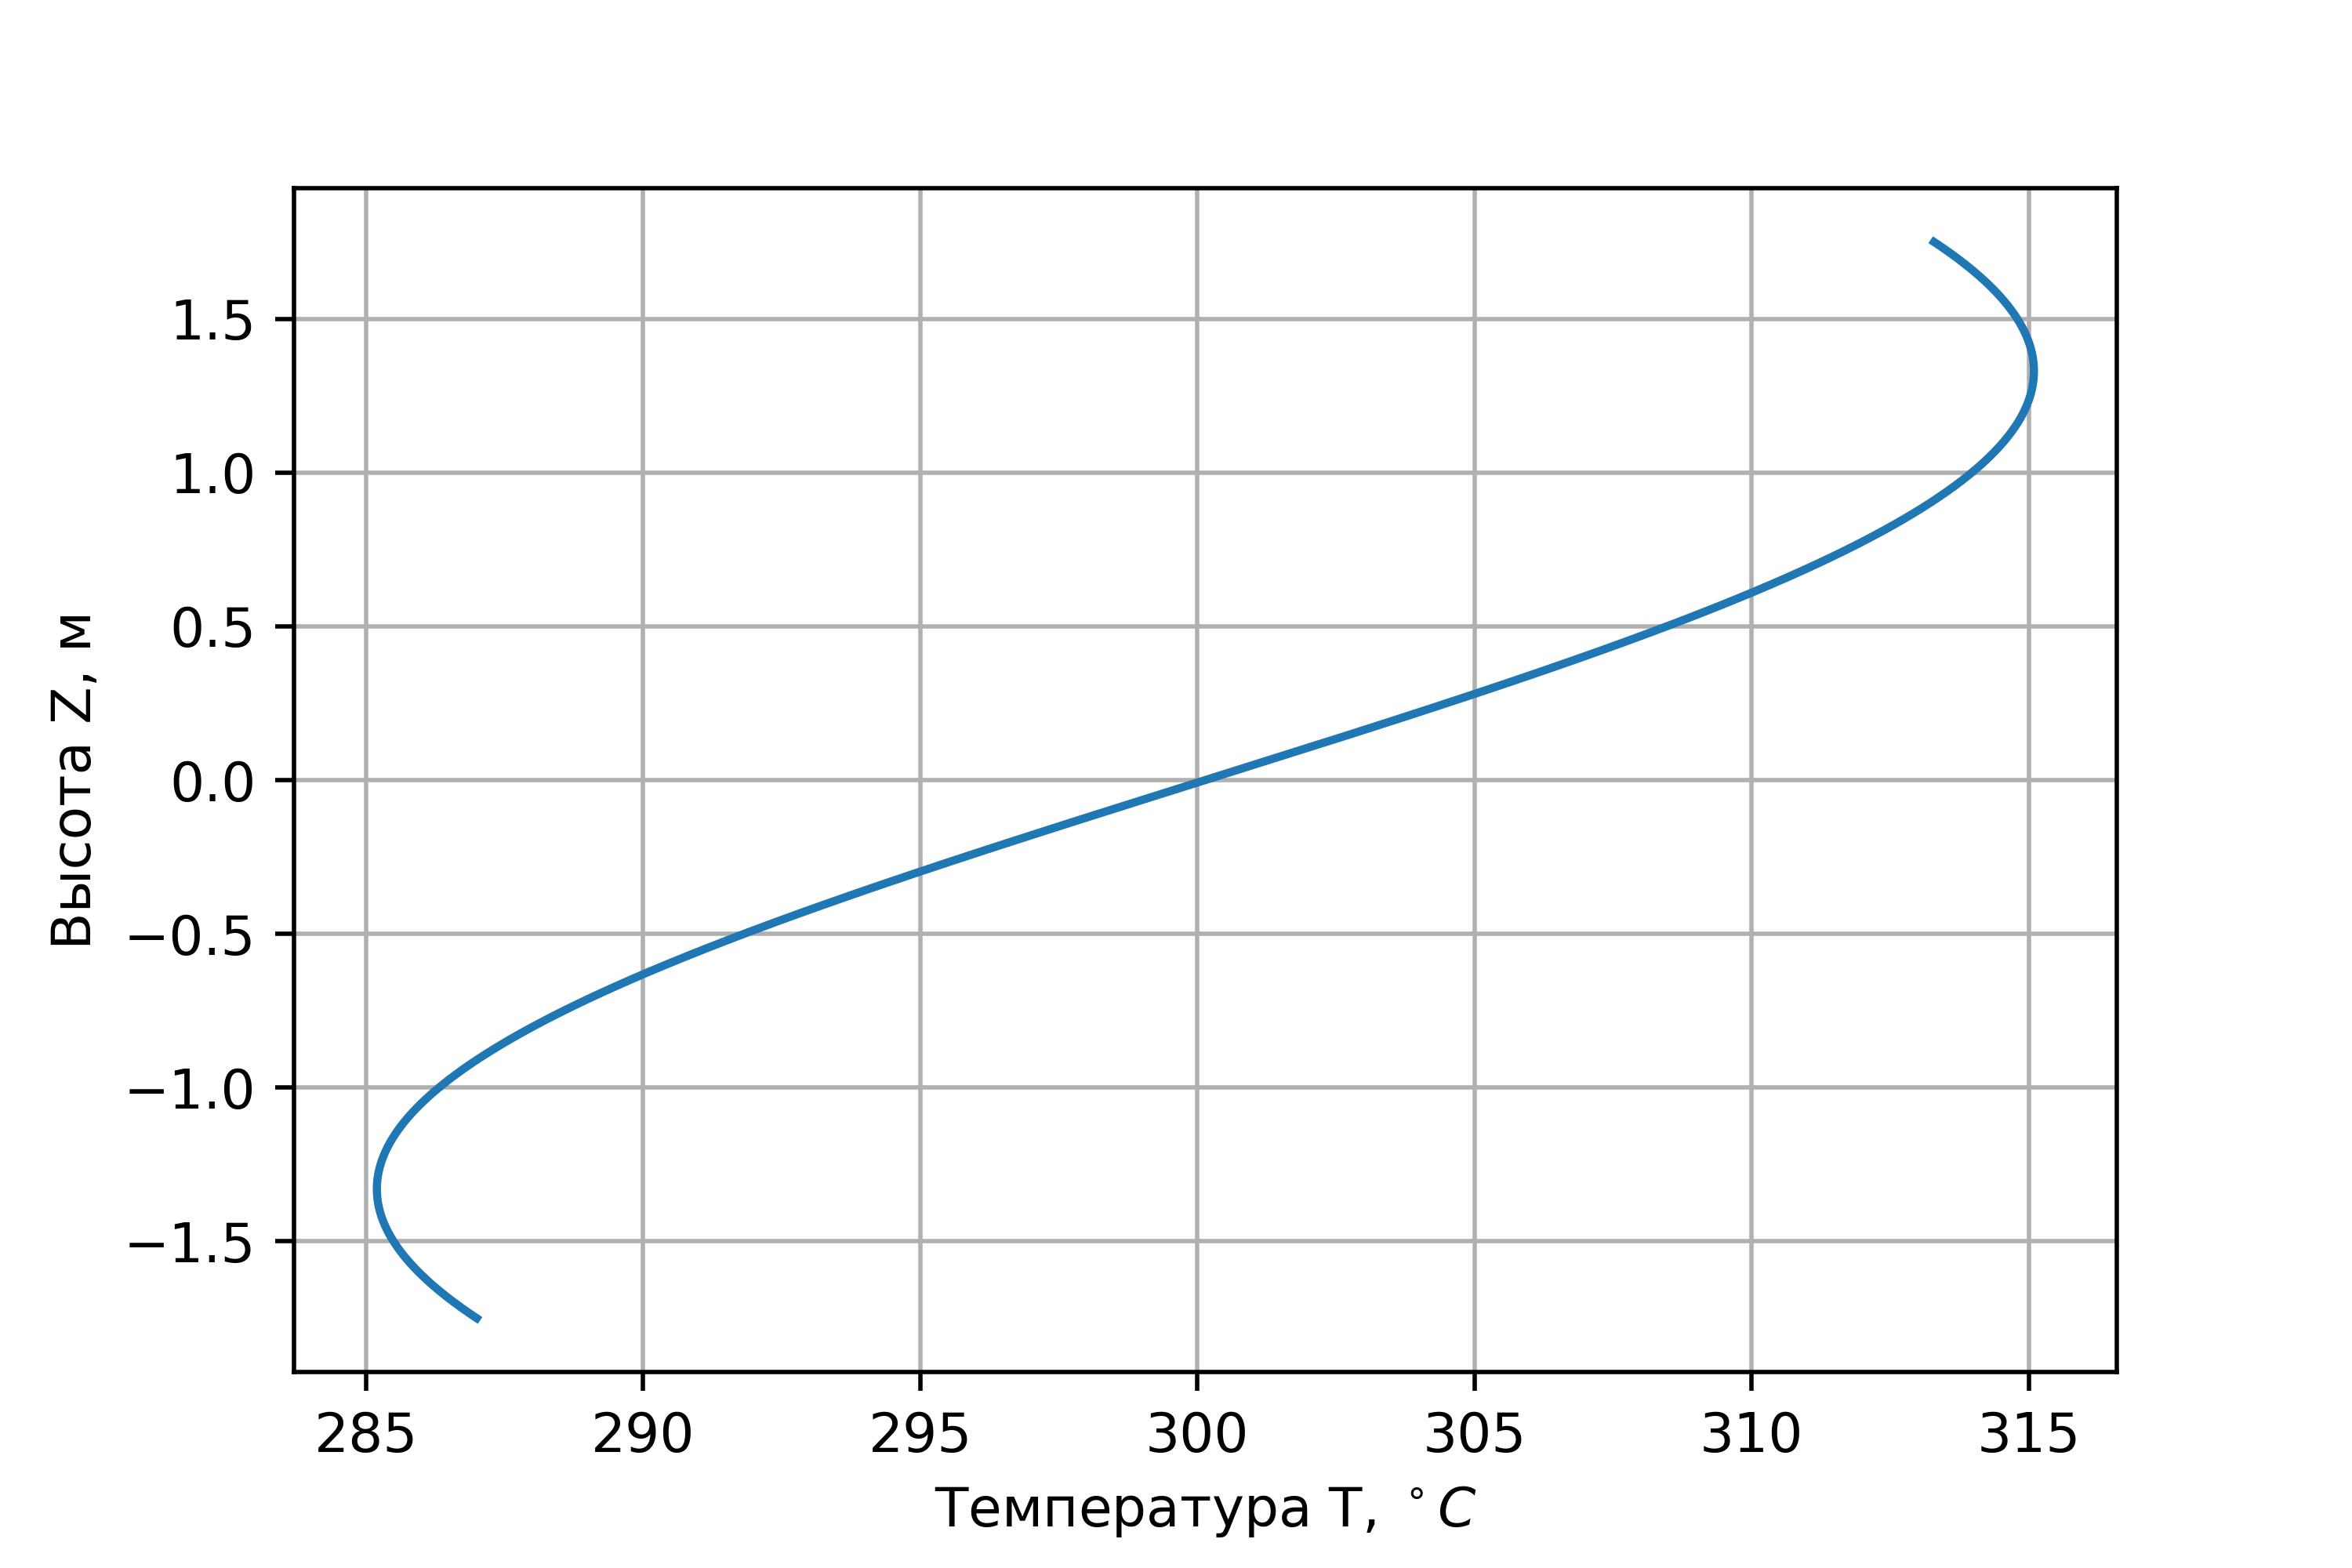
\includegraphics[]{Tz.png}
		\caption{Изменение температуры теплоносителя по высоте}
		\label{pic:TZ} % название для ссылок внутри кода
	\end{center}
\end{figure}

Максимальная температура теплоносителя определяется из температуры кипения теплоносителя при давлении в активной зоне. Температура насыщения воды при давлении $15.7$ МПа — $345.8\  ^\circ C$. Отсюда следует что запас до кипения $\approx 31 ^\circ C$. 

\subsection{Расчет распределения температуры внешней стенки оболочки по высоте}
Площадь проходного сечения:
$$
S_{\text{прох}} = \sqrt{3}/2(a - 2 \cdot \delta)^2 - N_{\text{твэл}} \frac {\pi d^2_{\text{тв}}} {4} - N_{\text{н.к.}} \frac {\pi D_{\text{н.к}}^2} {4} - \frac {D_{\text{ц.тр}}^2\pi}{4} = 2.4 \cdot 10^4\ \text{мм}^2
$$

Периметр:
$$
\Pi= (2(a-2\delta)\sqrt{3}) - N_{\text {твэл }} \pi d_{\text {тв }}+N_{\text {н.к }} \pi D_{\text {н.к }}+\pi D_{\text {ц.к}}= 10370 \text{мм}
$$
Гидравлический диаметр:
$$
d_{\text{Г}} = \frac {4 S_{\text{прох}}}{\text{П}} = 9.26 \text{мм} 
$$

Определим коэффициент теплоотдачи в режиме турбулентного
стационарного течения несжимаемой жидкости. По формуле Б.С.Петухова, В.В. Кириллова:
    Число Рейнолдса:
    $$
    \operatorname{Re}=\frac{G_{\text {pear }} \cdot d_{\mathrm{r}}}{N_{\mathrm{TBC}} \cdot S_{\text {npox }} \cdot \mu} = 5.15 \cdot 10^5
    $$
    Коэффициент гидравлического сопротивления:
    $$
    \xi=(1,82 \cdot \log (\mathrm{Re})-1.64)^{-2}= 0.013
    $$
    Расчитываем число Нуссельта:
    $$
    \mathrm{Nu}=\frac{\frac{\xi}{8} \cdot \mathrm{Re} \cdot \operatorname{Pr}}{k+12.7 \cdot\left(\operatorname{Pr}^{\frac{2}{3}}-1\right) \cdot \sqrt{\frac{\xi}{8}}} = 976.059 
    $$
    Коэффициент теплоотдачи:
    $$
    \alpha_1 = \frac {Nu \lambda_{\text{ср}}} {d_{\text{г}}} = 4.71 \cdot 10^4 \frac{\text{Вт}}{\text{м}^2 \cdot K}
    $$
    По формуле Диттуса-Болтера:
    $$
    Nu = 0.023Re^{0.8}Pr^{0.4} = 973.598
    $$
    Коэффициент теплоотдачи:
    $$
    \alpha_2 = \frac {Nu \lambda_{\text{ср}}} {d_{\text{г}}} = 4.69 \cdot 10^4 \frac{\text{Вт}}{\text{м}^2 \cdot K}
    $$
    По формула М.А. Михеева:
    $$
    Nu = 0.021Re^{0.8}Pr^{0.43} = 897.762
    $$
    Коэффициент теплоотдачи:
    $$
    \alpha_3 = \frac {Nu \lambda_{\text{ср}}} {d_{\text{г}}} = 4.33 \cdot 10^4 \frac{\text{Вт}}{\text{м}^2 \cdot K}
    $$
    Усредним коэффициент теплоотдачи:
    $$
    \alpha = \frac {\alpha_1 + \alpha_2 + \alpha_3} {3} = 4.58 \cdot 10^4 \frac{\text{Вт}}{\text{м}^2 \cdot K}
    $$
    Распределение температуры внешней стенки твэла по высоте реактора:
    $$
    T_{\text {об }}(z)=T_{\text {тн }}(z)+\frac{q_{\max } \cdot \cos \left(\frac{\pi \cdot z}{H_{\ni \phi}}\right)}{\pi d_{\text {тв }} \alpha}
    $$
Распределение температуры внешней стенки
твэла по высоте реактора представлено на \ref{pic:Tob}

\begin{figure}[H]
	\begin{center}
		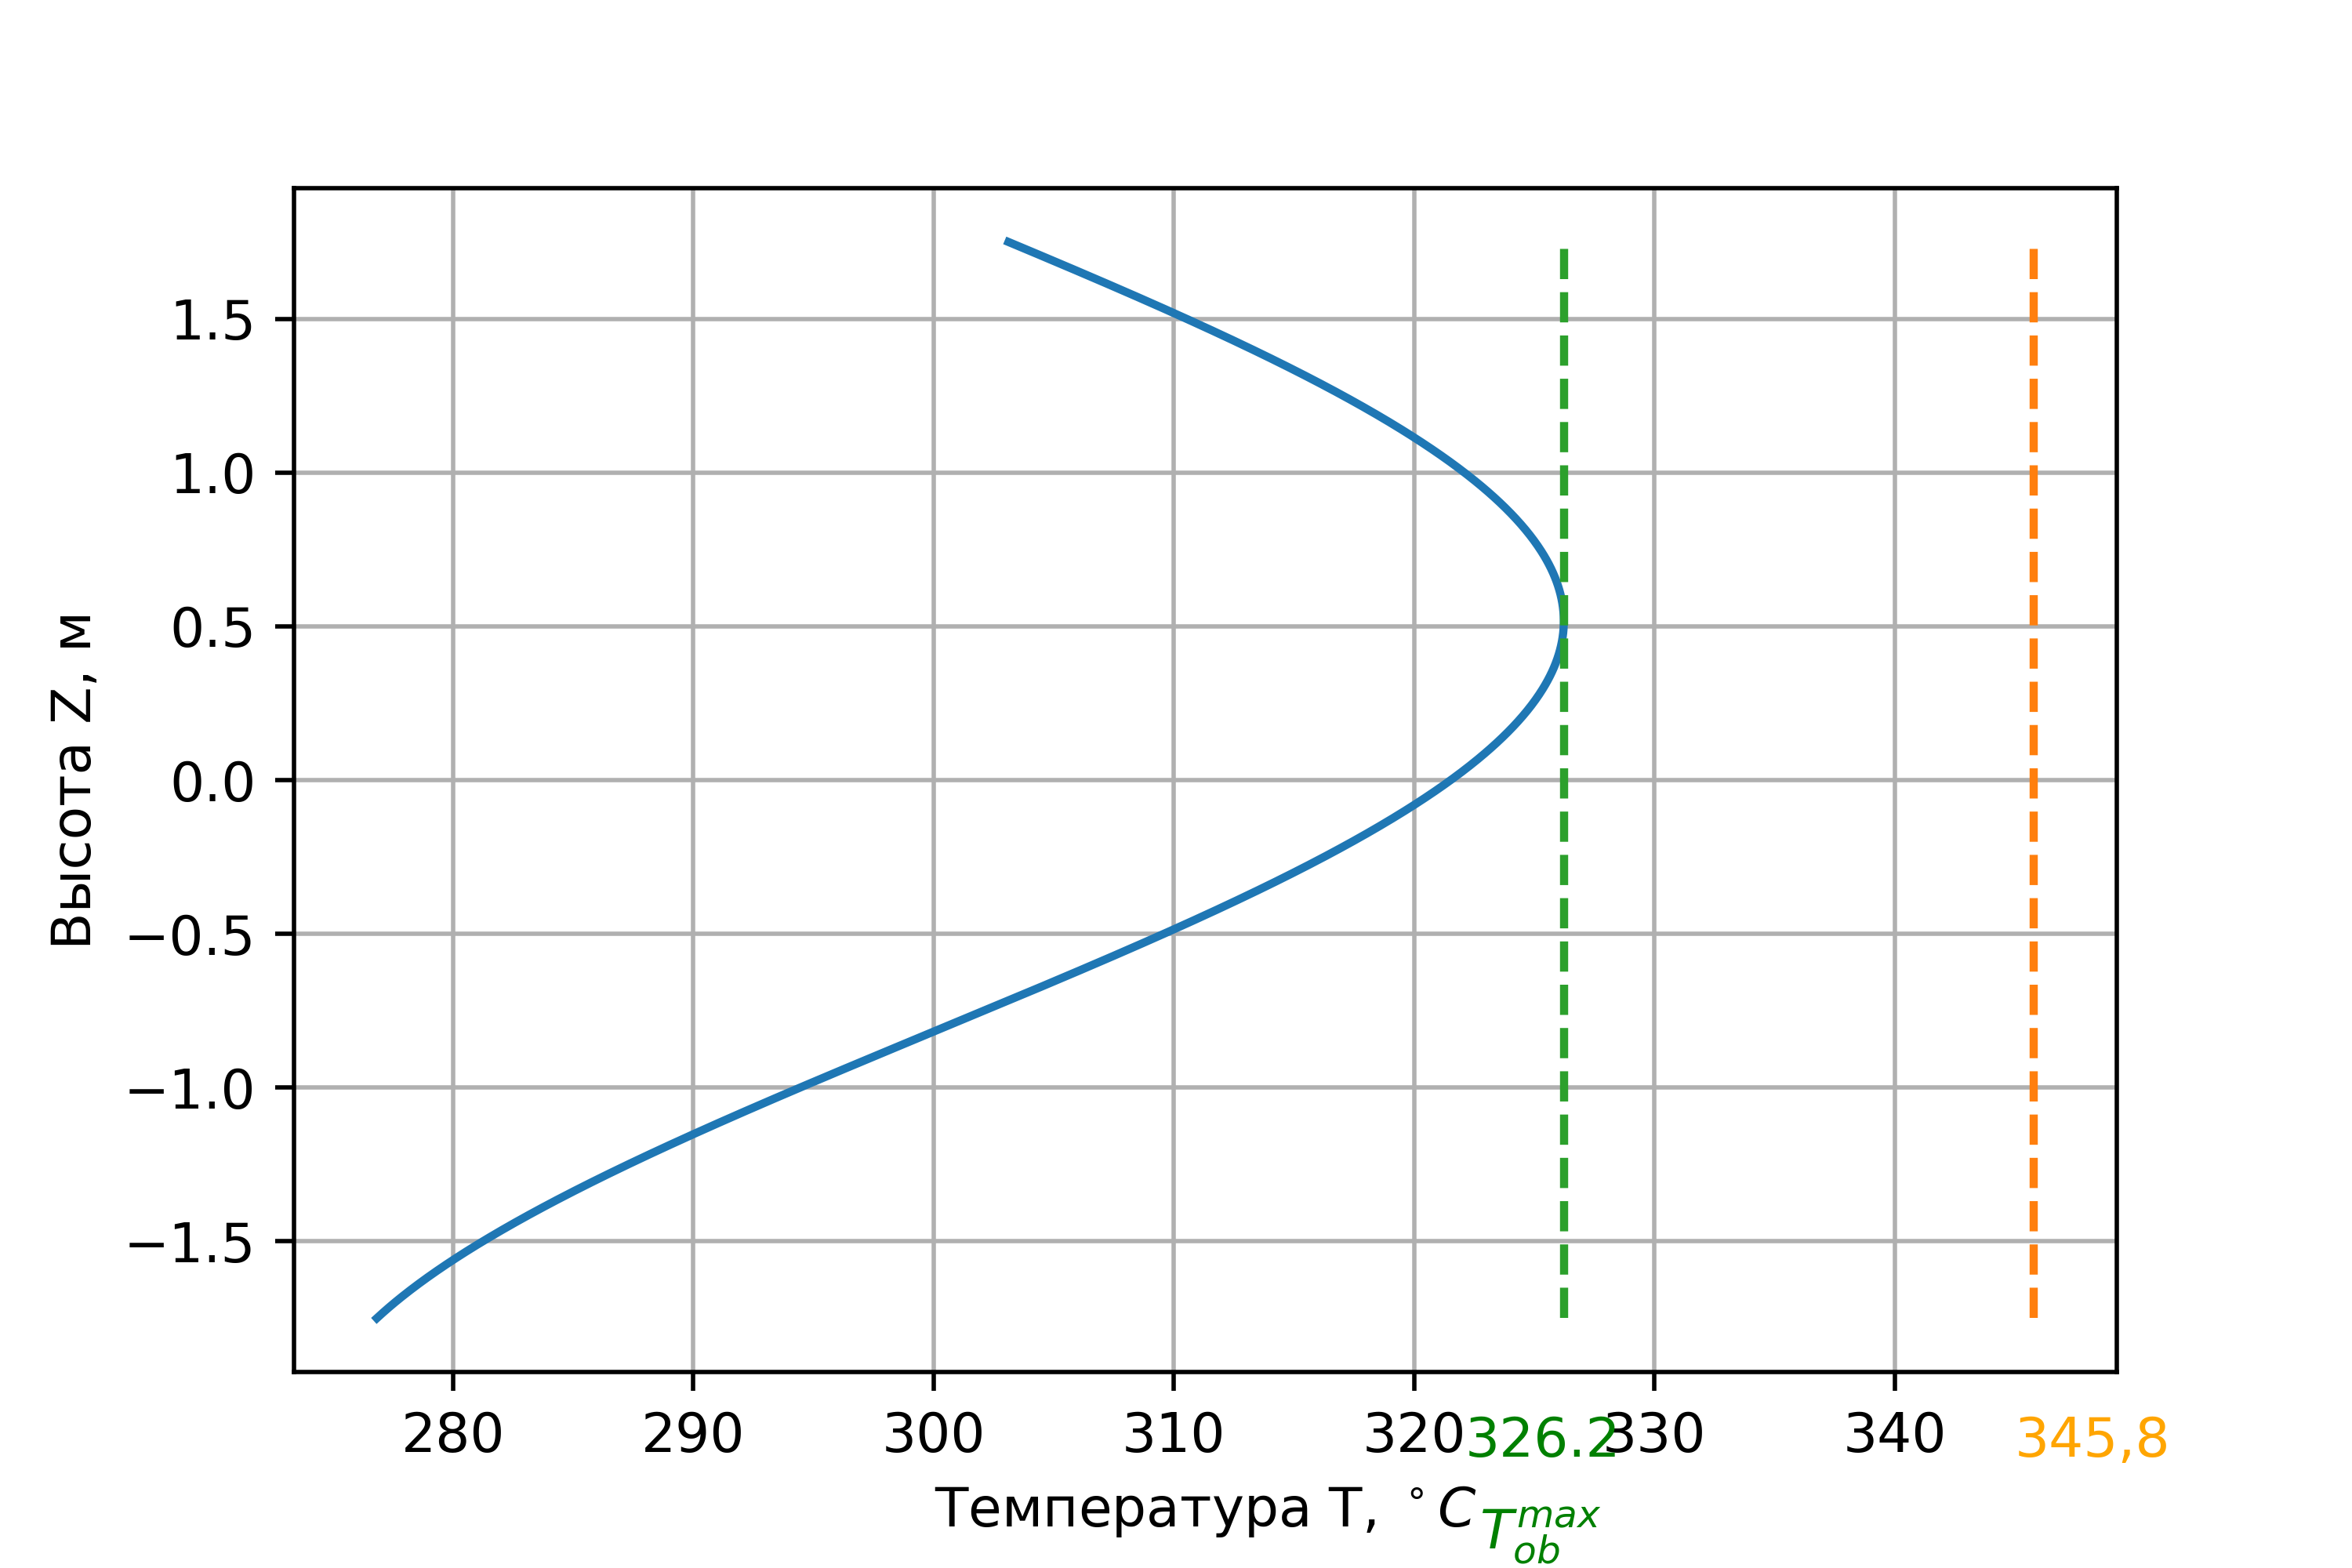
\includegraphics[]{Tob.png}
		\caption{Изменение температуры стенки твэла по высоте}
		\label{pic:Tob} % название для ссылок внутри кода
	\end{center}
\end{figure}

 Из \ref{pic:Tob} видно, что максимальная температура $T_{\text{об}}^{\max} = 326.2 ^\circ C $ стенки достигается в $Z_{\max} = 0.517 м$. Отсюда можно сделать вывод о том, что также отсутствует поверхностное кипения теплоносителя.
 %максимальная температура оболочки в условиях нормальной эксплуатации определяется прочностными и пластическими свойствами сплава и составляет сколь-кот то из справочника

% Общий график для распределений теплоносителя и оболочки представлены на \ref{pic:obsh}

% \begin{figure}[H]
	% \begin{center}
		% \includegraphics[]{Obsh.png}
		% \caption{Изменение температуры стенки твэла и теплоносителя по высоте}
		% \label{pic:obsh} % название для ссылок внутри кода
	% \end{center}
% \end{figure}
    
%NСУЗ — по числу отверстий в канале 

\subsection{Расчет температуры топлива}
    Произведём расчет термического сопротивления оболочки, газового зазора и топлива:
$$
\sum R_i = 
\frac {\ln \frac {d_{\text{тв}}}{d_{\text{тв}} - 2\delta_{ст}}  }{2\pi\lambda_{\text{об}}}+\frac {\ln \frac {d_{\text{тв}} - 2\delta_{ст}}{d_{\text{топ}}}  }{2\pi\lambda_{\text{г.з}}}+\frac {\frac 1 2 - \frac {d_{\text{отв}}^2} {d_{\text{топ}}^2 - d_{\text{отв}}^2}\ln \frac {d_{\text{топ}}}{d_{\text{отв}}}} {2 \pi \lambda_{\text{топ}}} = 0.04\  \frac{\text{м} \cdot \text{К}}{\text{Вт}}
$$
где
\begin{itemize}
    \item $\lambda_{\text{г.з.}} = 0.35\  \frac {\text{Вт}}{\text{м} \cdot \text{К}}$ — теплопроводность газового слоя 
    \item $\lambda_{\text{об}} = 23\  \frac {\text{Вт}}{\text{м} \cdot \text{К}}$ — теплопроводность оболочки 
    \item $\lambda_{\text{топ}} = 3\  \frac {\text{Вт}}{\text{м} \cdot \text{К}}$ — теплопроводность топлива
    \item $\delta_{\text{г.з}} =\frac {d_{\text{твэл}} - 2\delta_{\text{об}} - d_{\text{топ}}}{2} =  3\  \frac {\text{Вт}}{\text{м} \cdot \text{К}}$ — толщина газового зазора 
\end{itemize}
Распределение температур в топливе по высоте активной зоны:
$$
T_{\text {топ }}(z)=T_{\mathrm{cr}}(z)+\Sigma R_{i} \cdot q_{\max } \cdot \cos \left(\frac{\pi \cdot z}{H_{\text {эф }}}\right)
$$
График изменения температуры топлива по высоте представлен на \ref{pic:top}
\begin{figure}[H]
	\begin{center}
		\includegraphics[]{Ttop.png}
		\caption{Изменение температуры топлива по высоте}
		\label{pic:top} % название для ссылок внутри кода
	\end{center}
\end{figure}
\subsection{Определение перепадов давления и необходимой мощности насосов на прокачку}
Для того чтобы определить мощность на прокачку теплоносителя через реактор, найде перепад давления в ТВС
Гидравлическое сопротивление трения:
$$
\Delta P_{\text{тр}} = \frac 1 {2 d_{\text{г}}} \cdot \left(\frac {G_{\text{ТВС}}}{N_{\text{ТВС}}S_{\text{прох}}}  \right)^2 \cdot \frac {\xi_{\text{тр}}} {\rho_{\text{ср}}} = 1.363 \cdot 10^4 \text{Па}
$$
Потеря напора на ускорение:
$$
\Delta P_{\mathrm{уск}}=\left(\frac{G}{N_{\mathrm{TBC}} \cdot S_{\mathrm{npox}}}\right)^{2} \cdot\left(\frac{1}{\rho_{\mathrm{вых}}}-\frac{1}{\rho_{\mathrm{вx}}}\right) = 1.94 \cdot 10^3 \text{Па}
$$, где $\rho_{\text{вых}} = 680.8\  \frac {\text{кг}}{\text{м}^2} $, $\rho_{\text{вх}} =752.1\  \frac {\text{кг}}{\text{м}^2}$.
Нивелирный напор:
$$
\Delta P_{\text {нив }}=\left(\rho_{\text{вх}}-\rho_{\text{вых}}\right) \cdot g \cdot H_{\text{аз}}=2.45 \cdot 10^{3} \text{Па}
$$
Местное сопротивление:
$$
\Delta P_{\mathrm{мест}}=\frac{\left(\frac{G}{N_{\mathrm{TBC}} \cdot S_{\mathrm{прох}}}\right)^{2}}{2} \cdot\left(\frac{\xi_{\mathrm{вх}}}{\rho_{\mathrm{вх}}}+\frac{13 \xi_{\mathrm{pem}}}{\rho_{\mathrm{ср}}}+\frac{\xi_{\mathrm{вых}}}{\rho_{\mathrm{вых}}}\right)=
$$
где $\xi_{\text{вх}}= 2.6 $ — коэффициент сопротивления на входе в кассету; $\xi_{\text{вых}} = 0.45$ — коэффициент сопротивления при проходе через дистанцирующую решетку %укажи количество дистанцирующих решеток
Общее сопротивление каналов:
$$
\Delta P=\Delta P_{\mathrm{тр}}+\Delta P_{\mathrm{уск}}+\Delta P_{\text { нив }}+\Delta P_{\text {мест }} = 
$$
Мощность, необходимая для прокачки теплоносителя через весь реактор:
$$
N_{\mathrm{пр}}=N_{\mathrm{ТВС}} \frac{\Delta P \cdot G_{\mathrm{TBC}}}{\eta_{\text {нас }} \cdot \rho_{\mathrm{вх}}}=
$$
КПД реактора с учетом потерь на прокачку теплоносителя:
$$
\eta^{\prime}=\frac{Q_{\text {эл }}-N_{\text {пр }}}{Q_{\text {теп }}}
$$
% \subsection{Определение запаса до кризиса теплообмена}

\subsection{Выводы из теплофизического расчета}


% \section{Нейтронно-физический расчет}
